\chapter{Outlook \& Risk Assessment}
\label{chap:outlook}

\section{Risk Assessment}
\label{sec:RiskAssessment}

To reduce risks and increase the robustness within the development process for the INSPIRE mission, all subsystems focus on flight proven or space grade hardware. \autoref{tab:SubSys-TRL} provides an overview on the resulting TRL for each subsystem. 
 
\begin{table}[h]
\centering
\caption{Subsystem TRL for risk assessment}
\begin{tabular}{llll}
\toprule
Subsystem            & overall TRL & Deviating component      &  \\
\midrule
Payload              & 0           & Drill System and Sample Analyser TRL 0 &  \\
Structure \& Mechan. & 0           & Boom Mechanism TRL 0     &  \\
Locomotion           & 0-9           & Structure Components for Locomotion TRL 0                     &  \\
EPS                  & 9           & PCDU may be customised                     &  \\
TCS                  & 4-9           & none                     &  \\
COMs, C\&DH          & 9           & Housekeeping TRL 0       & 	 \\
\bottomrule
\end{tabular}
\label{tab:SubSys-TRL}
\end{table}

Housekeeping electronics and the boom mechanism to extend the camera head for the INSPIRE mission will be custom designed components and therefore rated at TRL 0. However due to proven development processes and simple testing the risk for the mission progress is rated non critical.  \\

Payload components development depict the highest risk for the mission. The Analyser for the ice core samples is a downsized replica of the APXS sensor \cite{ref_pay_1, ref_pay_2}. 
The ice core drill derives from the Nano Drill offered by Honeybee Robotics \cite{6497188}. Although the technology is available, the drill has to be adapted and tested. Testing in analog conditions potentially takes place in the arctic region and therefore lengthen the mission development process. \\

As a conclusion the payload subsystem development contains the highest risk for the INSPIRE mission. However the risk is considered manageable. Additionally investing in payload development is regarded worth the risk taking as it is integral to the successful investigation of Europa.

For the TCS the dimension of the  bi-metallic heat switches has to be adapted.
Tests in a special environment and for qualification have to be done as well. \\ \\
For the motors of the locomotion system, space grade components are selected. The stepper motors are already designed as space motors by Phytron \cite{Phytron}. The BLDCs of the wheel drive, on the other hand, were selected because the same series is also used in the Mars Rovers Curiosity. It should be noted, however, that these are special designs of the maxon company \cite{Maxon}. Therefore, no further data is available and the TRL, although already flight-proven, cannot be assumed to be 9. 

\clearpage

\section{Outlook}
\label{sec:Outlook}

In the further design iterations, detailed simulations of the chassis and the running gear could be carried out in order to get a better understanding of where the problems of the system are and at which points mass can possibly be reduced or should be added. It could also be considered whether a less complex mechanism for unfolding the drill can be designed. \\

Currently, the ice core samples taken be discarded after the analysis. It could be debated whether these samples will continue to be used. The previous considerations on this topic were, on the one hand, to store the samples and bring them back to the lander in order to be able to carry out further analyses if the lander should have a gripper arm or something similar to receive the samples or, on the other hand, to melt the samples and transport them to the Electric Bay with the help of micro-pumps in order to use the water gained in this way as protection against radiation. This could serve as a replacement for the previous solution and in the best case even save mass. \\

For the TCS, a more detailed analysis should to be carried out with the Finite-Element-Method to calculate the local heat and temperature distribution.
The FE results could be used to verify and adjust the analytical analysis to get a helpful tool for fast thermal calculation to evaluate different materials or designs in the further development phases.

\begin{figure}[htb]
     \centering
     \begin{subfigure}[b]{0.49\textwidth}
         \centering
         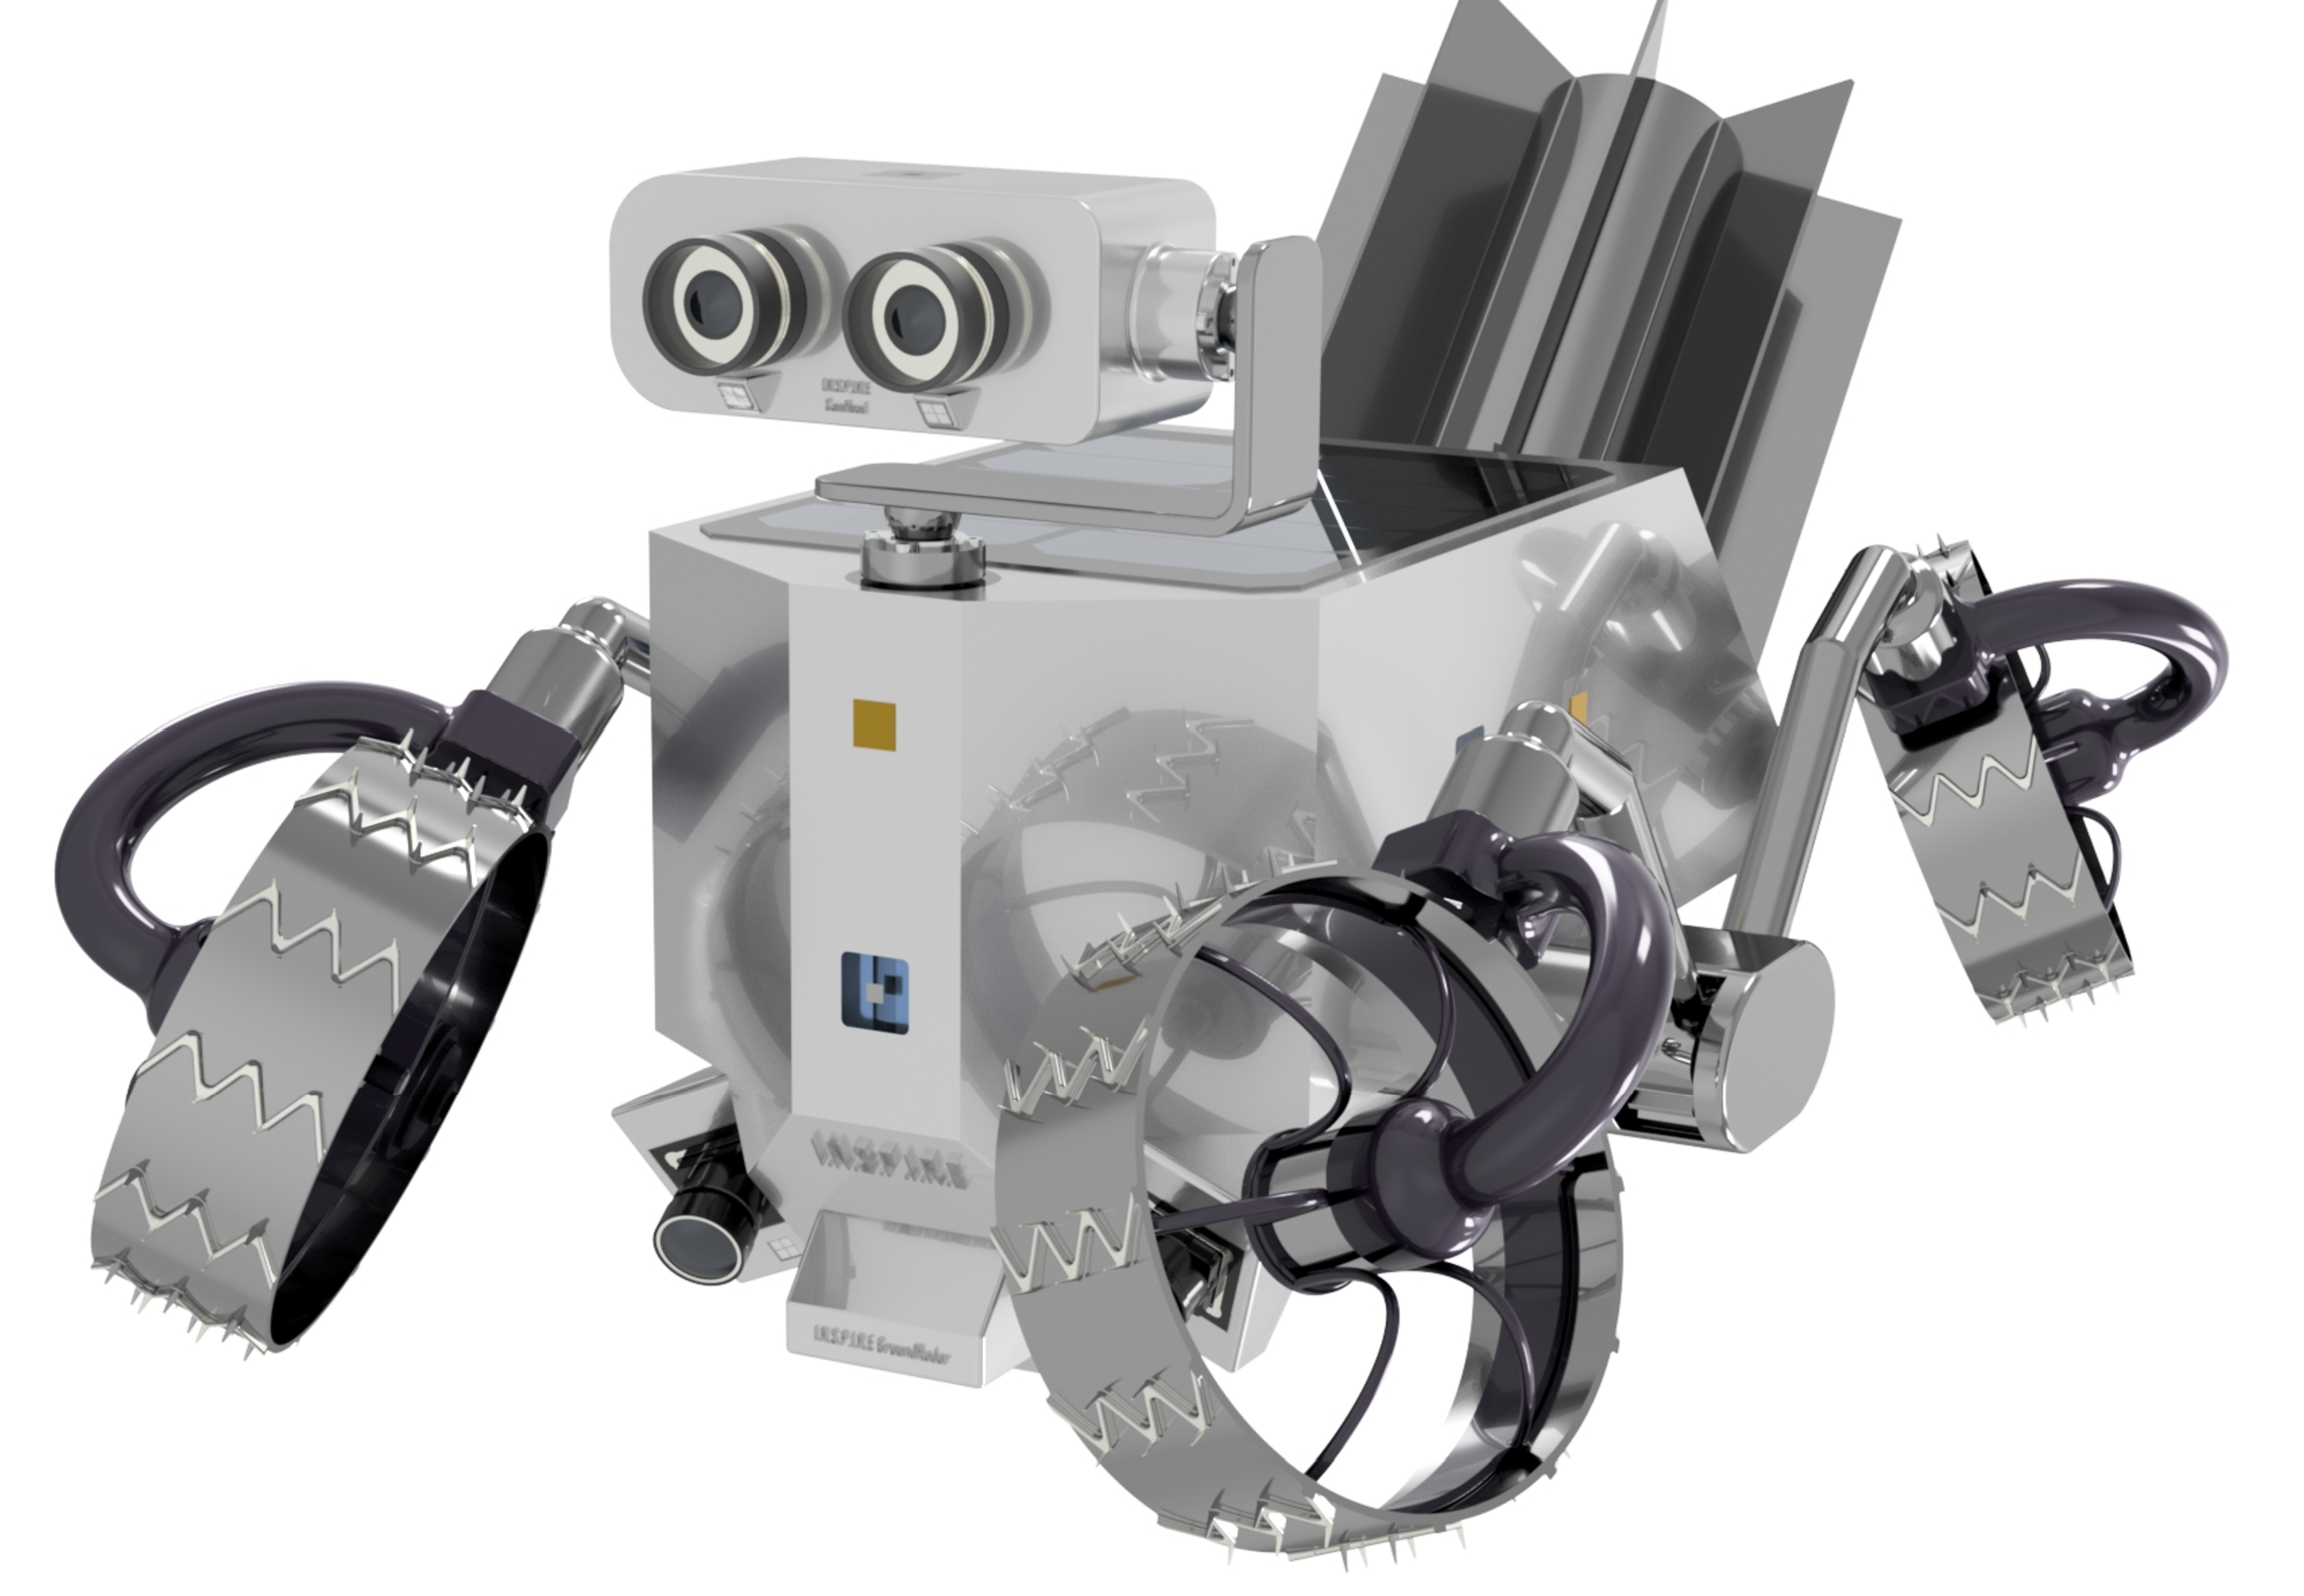
\includegraphics[width=\textwidth]{Media/INSPIRE Mk6_HighRes_Stowage_config}
         \caption{Storage Configuration}
         \label{fig:EndStorageConfig}
     \end{subfigure}
     \hfill
     \begin{subfigure}[b]{0.49\textwidth}
         \centering
         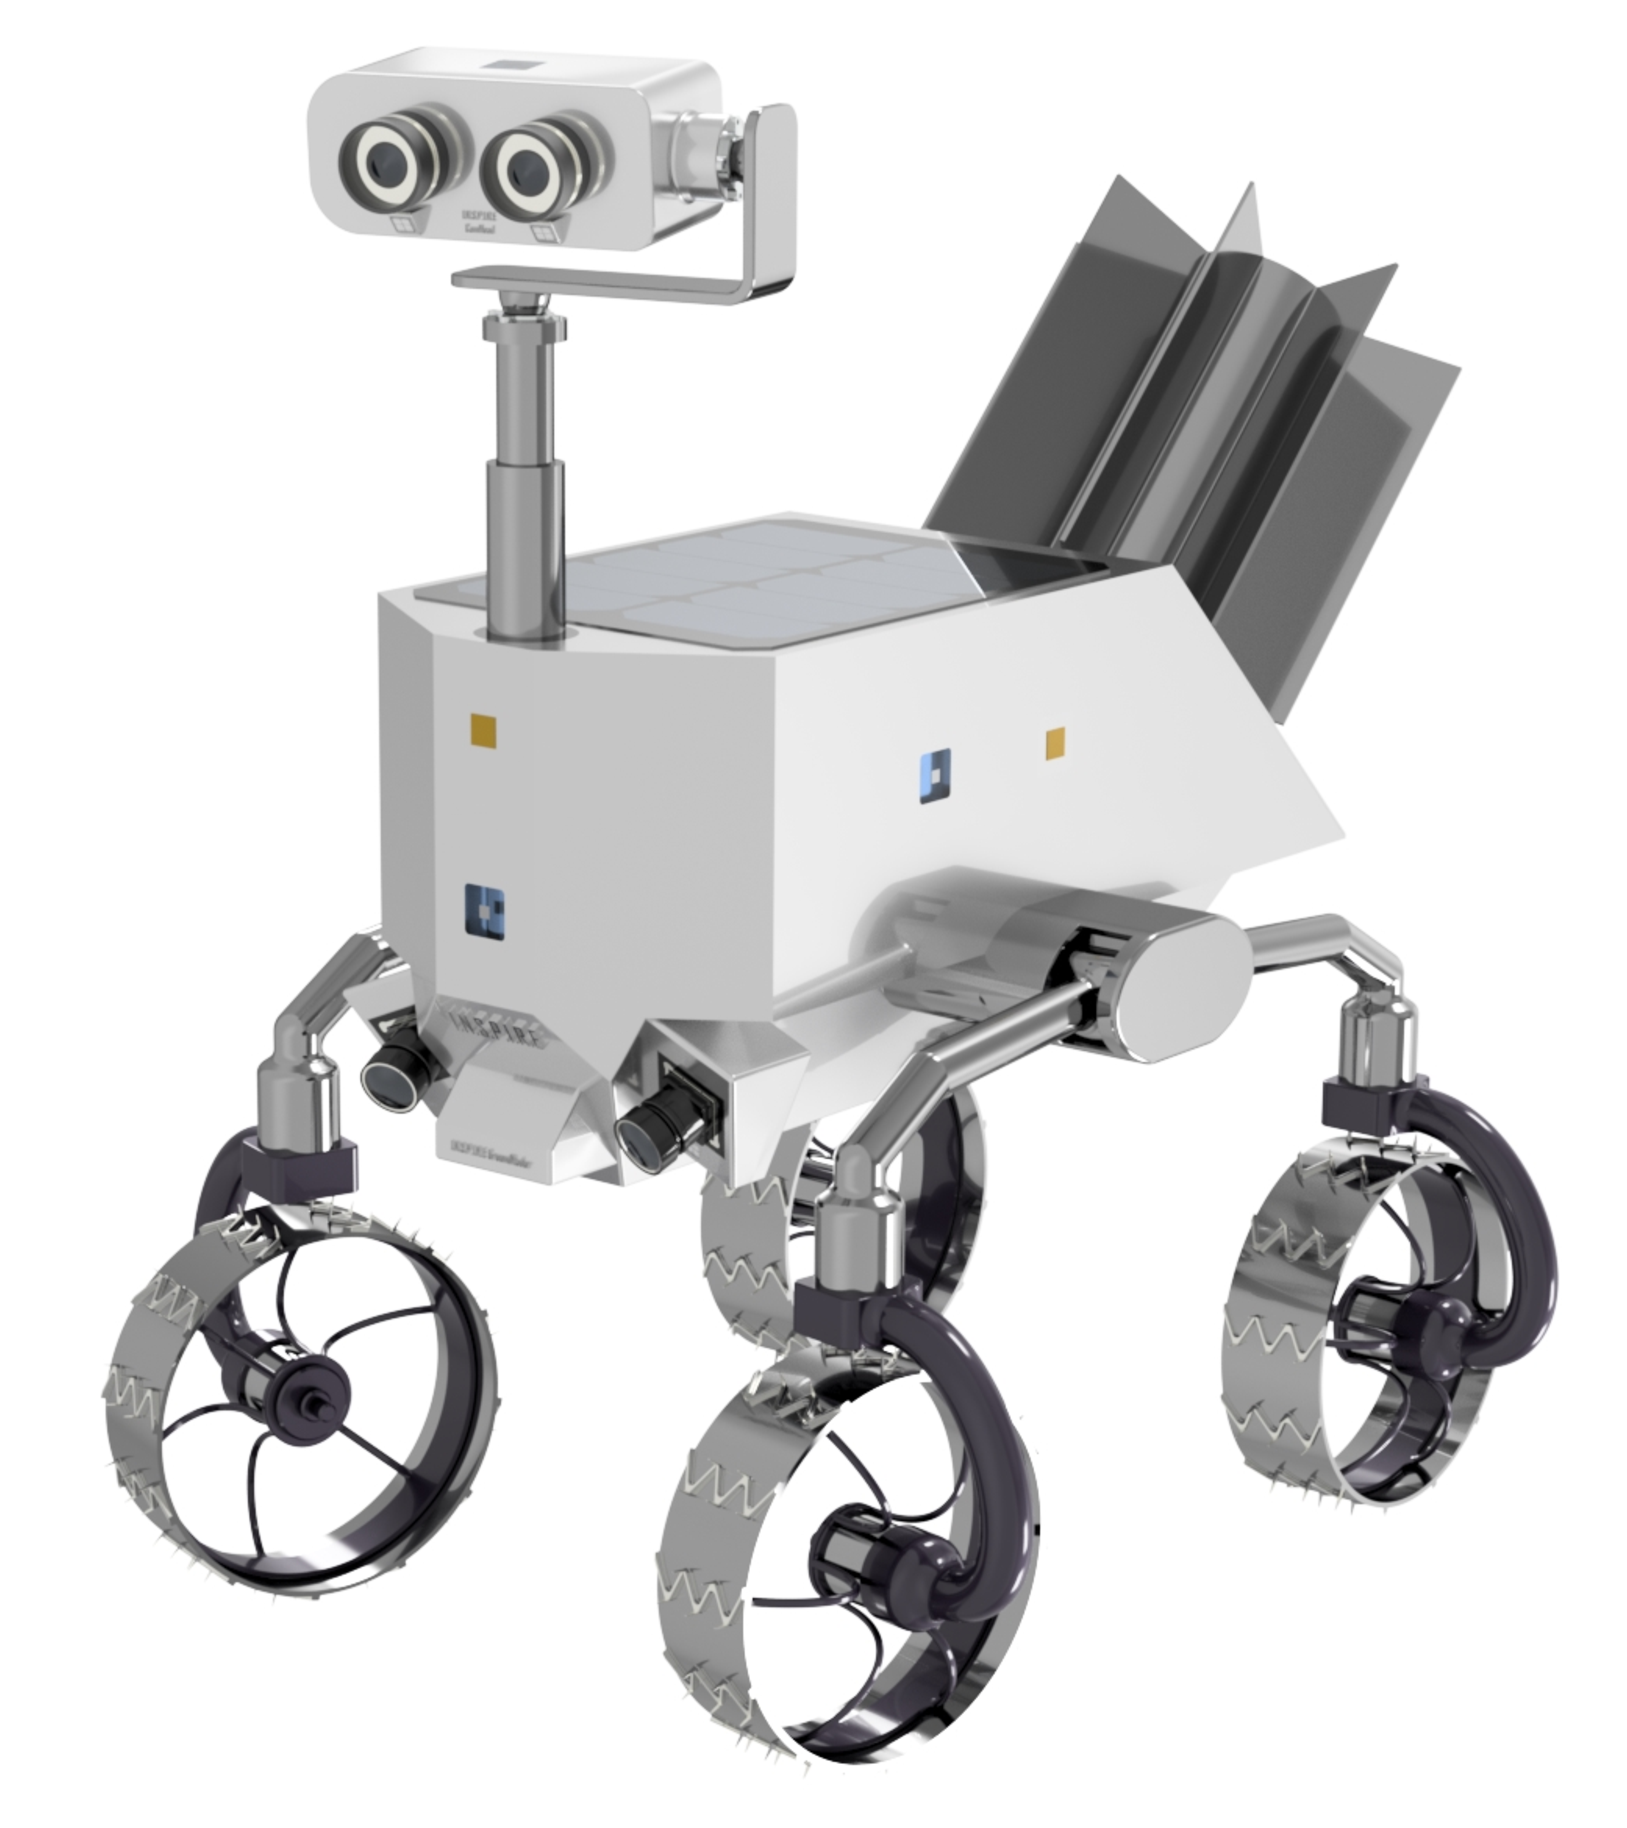
\includegraphics[width=\textwidth]{Media/INSPIRE Mk6_HighRes_Exploration}
         \caption{Exploration Configuration}
         \label{fig:EndExplorationConfig}
     \end{subfigure}
     \caption{The INSPIRE rover system in it's configurations}
     \label{fig:EndConfig}
\end{figure}

\clearpage